\documentclass[floatfix,nofootinbib,superscriptaddress,fleqn]{revtex4-2}  
%\documentclass[aps,epsfig,tightlines,fleqn]{revtex4}
\usepackage[utf]{kotex}
\usepackage[HWP]{dhucs-interword}
\usepackage[dvips]{color}
\usepackage{graphicx}
\usepackage{bm}
%\usepackage{fancyhdr}
%\usepackage{dcolumn}
\usepackage{defcolor}
\usepackage{amsmath}
\usepackage{amsfonts}
\usepackage{amssymb}
\usepackage{amscd}
\usepackage{amsthm}
\usepackage[utf8]{inputenc}
 \usepackage{setspace}
 \usepackage{tikz}
 \usepackage{pgf}
 
%\pagestyle{fancy}

\begin{document}

\title{\Large 2022년 1학기 물리학 I: Quiz 15}
\author{김현철\footnote{Office: 5S-436D (면담시간 매주
    화요일-16:00$\sim$20:00)}} 
\email{hchkim@inha.ac.kr}
\affiliation{Hadron Theory Group, Department of Physics,
Inha University, Incheon 22212, Republic of Korea }
\date{Spring semester, 2022}


\vspace{1.cm}

\maketitle


\noindent {\bf 문제 1. (30 pt)} 
그림~\ref{fig:1}처럼 질량 $m=0.85$ kg, 반지름 $r=4.2$ cm인 균일한 공이,
쓸림이 없는 벽에 고정되어있고 질량이 없는 줄에 매달려 있다. 공의
질량중심과 줄 끝 사이의 수직거리가 $L=8.0$ cm일 때
\begin{figure}[htp]
  \centering
\includegraphics[scale=0.5]{Qfig15-1-20220502.png}
  \caption{문제 1}
  \label{fig:1}
\end{figure}
\begin{itemize}
\item[(가)] 줄에 걸리는 장력과
\item[(나)] 벽이 공에 가하는 힘을 각각 구하여라. 
\end{itemize}

\noindent {\bf 풀이 : } 
공에 작용하는 수직항력 $N$, 중력 $F_g$, 장력 $T$, 자유 물체 다이어그램
\begin{figure}[htbp]
  \centering
  \begin{tikzpicture}
    \draw (0,-2.5) -- (0,2.5); 
    \draw (-2.5,0) -- (2.5,0);
    \draw [blue,very thick,-latex] (0.1,0)--(1.5,0) 
            node [above=2,black] {$T$};

    \draw[red,very thick,-latex] (0,-0.1) -- (0,-2) 
    node [left,black] {$F_g$};

    \draw[rotate=30,blue,very thick,-latex] (0,0.1)--(0,1.2)
    node [above,black] {$N$};
  \end{tikzpicture}
\end{figure} 

줄과 벽이 이루는 각도 $\theta$
운동 방정식
\begin{align}
  \label{eq:1-1}\sum F_x &= T-N\sin\theta =0, \\
  \label{eq:1-1-1}\sum F_y &= N\cos\theta -F_g =0.
\end{align}

\begin{itemize}
  \item[(가)] 식 \eqref{eq:1-1}, \eqref{eq:1-1-1}, $T$는,
  \begin{align}
    T = N\sin\theta=\frac{\sin\theta}{\cos\theta}F_g
    =\frac{\sin\theta}{\cos\theta}mg.
  \end{align}
$\theta$는,
\begin{align}
  \tan\theta = \frac{\sin\theta}{\cos\theta} = \frac{r}{L}.
\end{align}
따라서 $T$는,
\begin{align}
  \begin{split}
    T = \frac{r}{L}mg
  \end{split}
\end{align}

  \item[(나)]
  식 \eqref{eq:1-1-1},
  \begin{align}
    N =\frac{mg}{\cos\theta}
  \end{align}
\end{itemize}

\vspace{1.cm}

\noindent {\bf 문제 2. (30 pt)}
그림~\ref{fig:2}에서 바위를 타는 질량 55 kg인 사람이 손으로 바위틈 한
쪽을 잡아당기고 발로는 바위틈 반대쪽을 누르면서 ``뒤로 기대 오르기''를
하고 있다. 바위틈은 폭이 $w=0.20$ m이고, 사람의 질량 중심은 바위틈에서
수평으로 $d=0.40$ m의 거리에 있다. 정지마찰계수는 손과 바위 사이가
$\mu_1=0.40$이고 신발과 바위 사이는 $\mu_2=1.2$이다.  
\begin{figure}[ht]
  \centering
\includegraphics[scale=0.6]{Qfig15-2-20220502.png}
  \caption{문제 2}
  \label{fig:2}
\end{figure}
\begin{itemize}
\item[(가)] 사람이 안정되게 있기 위해서 손과 발이 각각 수평하게 가해야
  하는 최소한의 힘은 얼마인가?
\item[(나)] (가)와 같은 힘의 경우 손과 발 사이의 수직거리 $h$는
  얼마인가?
\item[(다)]  바위가 젖어서 $\mu_1$, $\mu_2$가 작아지면, (가)의
  답과
\item[(라)] (나)의 답은 어떻게 달라질까?
\end{itemize}

\noindent {\bf 풀이 : } 손에 작용하는 수직항력, 마찰력 $N_1$, $F_{s1}$, 발에 작용하는
수직항력, 마찰력 $N_2$, $F_{s2}$, 중력 $F_g$ 자유 물체 다이어그램

\begin{figure}[htbp]
  \centering
  \begin{tikzpicture}
    \draw (-2,2) node [] {$x$ 축 방향 : };
    \draw[blue,very thick,-latex] (0,-2)--(-2.4,-2)
    node [left,black] {$N_2$};
    \draw[blue,very thick,-latex] (0,1.6)--(1.6,1.6)
    node [right,black] {$N_1$};
    \draw[fill] (0,-2) circle (2pt) node [right,black] {$A$};
    \draw[thick] [|<->|] (0,-2)--(0,1.6) node [midway,left] {$h$};
  \end{tikzpicture}
  \centering
  \begin{tikzpicture}
    \draw (-2,2) node [] {$y$ 축 방향 : };
    \draw[fill] (-1.6,0) circle (2pt) node [above,black] {com};
    \draw[red,very thick,-latex] (-1.6,0) -- (-1.6,-2) 
    node [left,black] {$F_g$};
    \draw[red,very thick,-latex] (0.5,0)--(0.5,1.6)
    node [left,black] {$F_{s1}$};
    \draw[fill] (1.6,0) circle (2pt) node [below,black] {$A$};
    \draw[red,very thick,-latex] (1.6,0)--(1.6,1.6)
    node [right,black] {$F_{s2}$};
    \draw[thick] [|<->|] (-1.6,0)--(0.5,0) node [midway,below] {$d$};
    \draw[thick] [<->|] (0.5,0)--(1.6,0) node [midway,below] {$w$};
  \end{tikzpicture}
  \caption{자유 물체 다이어그램}
\end{figure} 

점 $A$는 발과 벽이 닿는 지점
운동 방정식,
\begin{align}
  \label{eq:2-1}\sum F_x &= N_{2}-N_{1} = 0,  \\
  \label{eq:2-1-1}\sum F_y &= F_{s1}+F_{s2}-F_g = 0.
\end{align}
\begin{itemize}
  \item[(가)] 마찰력은 수직항력에 비례하므로,
  \begin{align}
    F_{s1} = \mu_1N_1,\,\,\,
    F_{s2} = \mu_2N_2.
  \end{align}
  아이는 정지해있으므로 식 \eqref{eq:2-1}, \eqref{eq:2-1-1}에 의해,
  \begin{align}
    N_{2} = N_{1},\,\,\,F_{s1}+F_{s2}=F_g.
  \end{align}
  따라서,
  \begin{align}
    F_{s1}+F_{s2}= \mu_1N_1+\mu_2N_2= (\mu_1+\mu_2)N_1 =F_g.
  \end{align}
  최소한의 $N_1$은 중력 보다 커야하므로,
  \begin{align}\label{eq:2-2}
    N_1 \geq \frac{mg}{\mu_1+\mu_2}.
  \end{align}
  \item[(나)] 
  사람은 정지해있으므로 돌림힘 $0$, 점 $A$를 회전축으로 하는
  돌림힘 계산
  \begin{align}
    \sum \tau = N_1 h + F_{s1} w - F_g(w+d) = 0
  \end{align}
  $h$에 대해 정리하면
  \begin{align}\label{eq:2-3}
    h = \frac{F_g(w+d)-F_{s1} w}{N_1}
    =\frac{mg(w+d)-\mu_1N_1 w}{N_1}
  \end{align}
  수치를 넣어 값을 계산
  \item[(다)]
  식~\eqref{eq:2-2}로 부터
  \item[(라)]
  식~\eqref{eq:2-3}로 부터
\end{itemize}

\vspace{1.cm}



\noindent {\bf 문제 3. (60pt)  {\color{red} 난이도 상}:} 
질량 $m_b$, 길이 $L$인 수평하고 균일한 막대가 왼쪽은 경첩으로 벽에
붙어 있고, 오른쪽은 수평과 각도 $\theta$인 줄로 매여 있는 걸
그림~\ref{fig:3}a에서 보여준다. 질량 $m_p$인 물체가 왼쪽 끝에서부터
$x$인 위치에 얹혀 있고, 전체 질량은 $m_b+m_p=61.22$
kg이다. 그림~\ref{fig:3}b는 줄의 장력을 물체의 위치 $x/L$의 함수로
나타낸 것이다. $T$ 축의 눈금은 $T_a=500$ N, $T_b=700$ N으로 나타낸다. 
\begin{figure}[htbp]
  \centering
\includegraphics[scale=0.4]{Qfig15-3-20220502.png}
  \caption{문제 3}
  \label{fig:3}
\end{figure}
\begin{itemize}
\item[(가)] 각도 $\theta$
\item[(나)] 질량 $m_b$
\item[(다)] 질량 $m_p$를 각각 구하여라. 
\end{itemize}

\noindent {\bf 풀이 : } 

\begin{figure}[htbp]
  \centering
  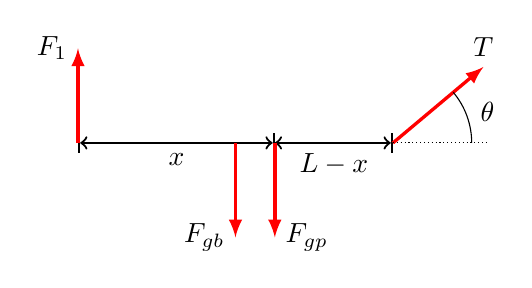
\begin{tikzpicture}
    
    \coordinate (A) at (-2,0);
    \coordinate (b) at (0,0);
    \coordinate (p) at (0.5,0);
    \coordinate (B) at (2,0);
    \draw[thick] [|<->|] (A)--(p) node [midway,below] {$x$};
    \draw[thick] [<->|] (p)--(B) node [midway,below] {$L-x$};
    \draw[red,very thick,-latex] (A)-- +(0,1.2)
    node [left,black] {$F_1$};
    \draw[red,very thick,-latex] (b)-- +(0,-1.2)
    node [left,black] {$F_{gb}$};
    \draw[red,very thick,-latex] (p)-- +(0,-1.2)
    node [right,black] {$F_{gp}$};
    \draw[red,very thick,-latex] (B)-- +(40:1.5)
    node [above,black] {$T$};
    \draw[densely dotted] (B)-- +(1.2,0);
    \draw[] (B)+(1,0) arc(0:40:1) (B)+(1.2,0.4)
    node[] {$\theta$};
    % \draw[fill] (-1.6,0) circle (2pt) node [above,black] {com};
    % \draw[red,very thick,-latex] (-1.6,0) -- (-1.6,2) 
    % node [left,black] {$F_g$};
    % \draw[red,very thick,-latex] (0.5,0)--(0.5,-1.6)
    % node [left,black] {$F_{s1}$};
    % \draw[fill] (2,0) circle (2pt) node [below,black] {$A$};
    % \draw[red,very thick,-latex] (0.2,0)--(0.2,-1.6)
    % node [below,black] {$F_{s2}$};

    % \draw[thick] [<->|] (0.5,0)--(2,0) node [midway,below] {$L-x$};
  \end{tikzpicture}
  \caption{자유 물체 다이어그램}
\end{figure} 

경첩에 의한 수직항력 $F_1$, 물체에 의한 중력 $F_{gb}$, 막대에 의한 중력 $F_{gp}$,
케이블에 의한 장력 $T$
그래프를 수식적으로 표현해보면
\begin{align}
  T = \left(\frac{T_b - T_a}{1-0}\right)\frac{x}{L}+T_a
  =\left(T_b - T_a\right)\frac{x}{L}+T_a
\end{align}
경첩을 회전축으로 하는 돌림힘 계산

\begin{itemize}
  \item[(가)]
  \item[(나)]
  \item[(다)]
\end{itemize}
\vspace{1.cm}

\noindent {\bf 풀이 : } 

\noindent {\bf 문제 4. (40pt)}
그림~\ref{fig:4}는 질량 103 kg인 균일한 통나무를 반지름 1.20 mm인 두
개의 강철선 $A$와 $B$로 매달아 놓은 것이다. 처음에는 길이가 2.50 m인
줄 $A$가 줄보다 2.00 mm만큼 짧았으나 지금은 통나무가 수평하게 되었다. 
$B$보다 
\begin{figure}[ht]
  \centering
\includegraphics[scale=0.25]{Qfig15-4-20220502.png}
  \caption{문제 4}
  \label{fig:4}
\end{figure}
\begin{itemize}
\item[(가)] 줄 $A$와
\item[(나)] 줄 $B$가 통나무에 가하는 힘은 각각 얼마인가? 
\item[(다)] $d_A/d_B$의 비율은 얼마인가? 
\end{itemize}

\noindent {\bf 풀이 : } 
\begin{itemize}
  \item[(가)]
  \item[(나)]
  \item[(다)]
\end{itemize}

\end{document}